% ============================================================
%  Section 6.2 – Communication Protocols
% ============================================================
\section{Communication Protocols}
\label{sec:ch6_comms}

The two-site deployment relies on a layered communication stack in which each layer addresses a
distinct class of data.  Figure~\ref{fig:ch6_comms_stack} shows how these layers are assembled on
top of the ZeroTier virtual overlay described in Section~\ref{sec:zerotier_overlay}.

% ------------------------------------------------------------------
%  Figure: layered communication stack (TikZ)
% ------------------------------------------------------------------
\begin{figure}[H]
\centering
\begin{tikzpicture}[
    font=\small\sffamily,
    box/.style={
        draw, rounded corners=4pt, minimum width=10cm, minimum height=0.85cm,
        align=center, text width=9.5cm
    },
    label/.style={font=\footnotesize\sffamily\itshape, text=gray}
]

% Layer 0 – physical internet
\node[box, fill=gray!15] (inet) at (0,0)
    {Public Internet (physically distinct LANs, NAT boundaries)};

% Layer 1 – ZeroTier overlay
\node[box, fill=cyan!20, above=0.35cm of inet] (zt)
    {ZeroTier Virtual Overlay \quad|\quad Stable unicast IP, AES-256 tunnel};

% Layer 2A – Fast DDS / RTPS
\node[box, fill=orange!25, above=0.35cm of zt] (dds)
    {Fast DDS / RTPS (ROS~2 middleware) \quad|\quad
     Static unicast discovery, QoS profiles};

% Layer 2B – Syncthing (sits beside DDS)
\node[box, fill=teal!20, above=0.35cm of dds] (sync)
    {Syncthing file-sync channel \quad|\quad
     Program-storage YAML, encrypted P2P over ZeroTier};

% Layer 3 – ROS 2 application
\node[box, fill=blue!20, above=0.35cm of sync] (app)
    {ROS~2 Application Layer \quad|\quad
     Topics, Services, Actions, QoS-annotated publishers/subscribers};

% Arrows
\foreach \a/\b in {inet/zt, zt/dds, dds/sync, sync/app}
    \draw[->, thick] (\a.north) -- (\b.south);

% Side labels
\node[label, right=0.3cm of inet]  {physical};
\node[label, right=0.3cm of zt]    {network};
\node[label, right=0.3cm of dds]   {real-time};
\node[label, right=0.3cm of sync]  {file-sync};
\node[label, right=0.3cm of app]   {application};

\end{tikzpicture}
\caption{Layered communication stack used by the dual-laptop deployment.}
\label{fig:ch6_comms_stack}
\end{figure}

% ------------------------------------------------------------------
\subsection{Real-Time Channel: Fast DDS over ZeroTier}
\label{subsec:ch6_fastdds}
% ------------------------------------------------------------------

ROS~2 Jazzy uses \textbf{eProsima Fast DDS} (\texttt{rmw\_fastrtps\_cpp}) as its default
middleware.  RTPS normally relies on IP multicast for participant discovery, which does not
cross NAT or subnet boundaries.  Three configuration changes, supplied via an XML participant
profile pointed to by the \texttt{FASTRTPS\_DEFAULT\_PROFILES\_FILE} environment variable,
adapt the stack to the ZeroTier overlay:

\begin{enumerate}
    \item \textbf{Disable multicast discovery.}  The \texttt{<metatrafficMulticastLocatorList>}
          is left empty and replaced with explicit \texttt{<initialPeersList>} entries that list
          each peer's ZeroTier virtual IP address.

    \item \textbf{Bind to the ZeroTier interface.}  An \texttt{<interfaceWhiteList>} entry
          restricts Fast~DDS to advertise and receive on the \texttt{ztXXXXXXXX} interface only,
          preventing the physical Wi-Fi addresses (which are unreachable from the remote site)
          from appearing in RTPS locator lists.

    \item \textbf{Per-topic QoS profiles.}  Table~\ref{tab:ch6_qos} summarises the reliability
          and durability contracts applied to each data stream.
\end{enumerate}

% ------------------------------------------------------------------
%  Figure: Fast DDS unicast discovery sequence (TikZ sequence diagram)
% ------------------------------------------------------------------
\begin{figure}[H]
\centering
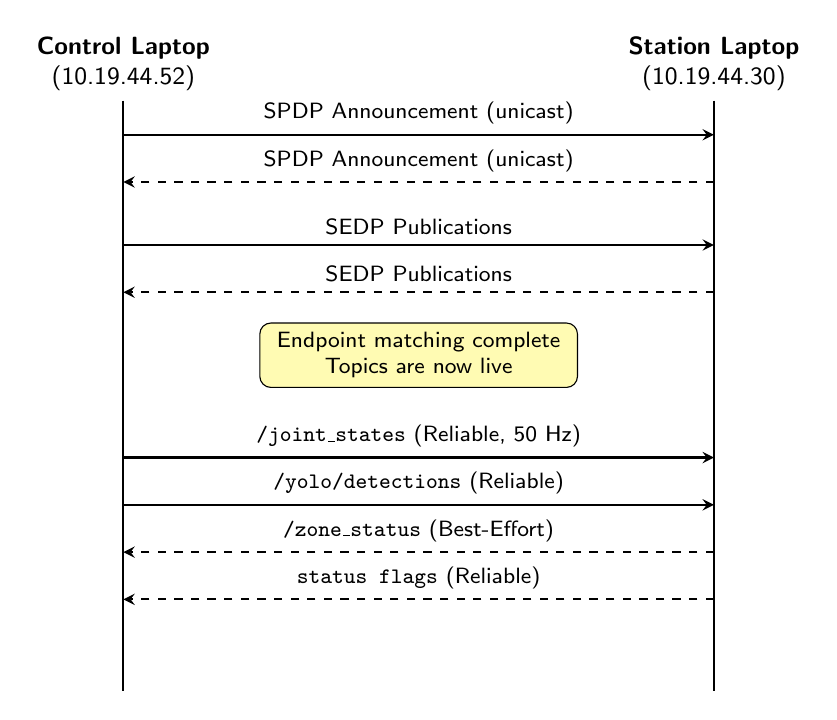
\begin{tikzpicture}[
    font=\small\sffamily,
    node distance=6cm,
    lifeline/.style={thick},
    msg/.style={->, >=stealth, thick},
    retmsg/.style={->, >=stealth, thick, dashed},
    lbl/.style={font=\footnotesize\sffamily}
]

% Participants
\node[align=center] (ctrl) at (0,0)    {\textbf{Control Laptop}\\(10.19.44.52)};
\node[align=center] (stat) at (7.5,0)  {\textbf{Station Laptop}\\(10.19.44.30)};

% Lifelines
\draw[lifeline] (ctrl.south) -- ++(0,-7.5);
\draw[lifeline] (stat.south) -- ++(0,-7.5);

% Time markers
\def\y{-0.6}

% SPDP
\draw[msg] (0,\y-0.3) -- node[above, lbl]{SPDP Announcement (unicast)} (7.5,\y-0.3);
\draw[retmsg] (7.5,\y-0.9) -- node[above, lbl]{SPDP Announcement (unicast)} (0,\y-0.9);

% SEDP
\draw[msg] (0,\y-1.7) -- node[above, lbl]{SEDP Publications} (7.5,\y-1.7);
\draw[retmsg] (7.5,\y-2.3) -- node[above, lbl]{SEDP Publications} (0,\y-2.3);

% Matched note
\node[draw, rounded corners, fill=yellow!30, font=\footnotesize\sffamily,
      text width=3.8cm, align=center] at (3.75,-3.7)
    {Endpoint matching complete\\Topics are now live};

% Topic data
\draw[msg] (0,\y-4.4) -- node[above, lbl]{\texttt{/joint\_states} (Reliable, 50~Hz)} (7.5,\y-4.4);
\draw[msg] (0,\y-5.0) -- node[above, lbl]{\texttt{/yolo/detections} (Reliable)} (7.5,\y-5.0);
\draw[retmsg] (7.5,\y-5.6) -- node[above, lbl]{\texttt{/zone\_status} (Best-Effort)} (0,\y-5.6);
\draw[retmsg] (7.5,\y-6.2) -- node[above, lbl]{\texttt{status flags} (Reliable)} (0,\y-6.2);

\end{tikzpicture}
\caption{Fast~DDS unicast discovery and topic flow between the two laptops.}
\label{fig:ch6_dds_discovery}
\end{figure}

% ------------------------------------------------------------------
%  Table: per-stream QoS profiles
% ------------------------------------------------------------------
\begin{table}[H]
\centering
\caption{QoS profiles assigned to each ROS~2 data stream.}
\label{tab:ch6_qos}
\setlength{\tabcolsep}{6pt}
\begin{tabular}{llll}
\toprule
\textbf{Topic / Stream} & \textbf{Reliability} & \textbf{Durability} & \textbf{Target Rate} \\
\midrule
\texttt{/joint\_states}           & Reliable    & Volatile      & 50 Hz  \\
\texttt{/yolo/detections}         & Reliable    & Volatile      & 10 Hz  \\
\texttt{/zone\_status}            & Best-Effort & Volatile      & 2 Hz   \\
\texttt{status flags}             & Reliable    & Transient Local & on change \\
\texttt{/twin/divergence}         & Best-Effort & Volatile      & 10 Hz  \\
\texttt{/dt/program\_status}      & Reliable    & Transient Local & on change \\
\bottomrule
\end{tabular}
\end{table}

The \emph{Reliable} contract is used wherever a missed message could corrupt the system state
(joint feedback, program events).  \emph{Best-Effort} is acceptable for diagnostic streams such
as divergence values and zone indicators, where a single skipped sample is inconsequential.

% ------------------------------------------------------------------
\subsection{File-Sync Channel: Syncthing for Program-Storage Transfer}
\label{subsec:ch6_syncthing}
% ------------------------------------------------------------------

The execution program — a YAML file holding the validated joint trajectories — is regenerated
only when the operator commits a new plan.  Forcing this document through a publish-subscribe
topic would waste DDS bandwidth on an infrequent, large payload while adding unnecessary
complexity to the subscriber code.  Instead, the system uses \textbf{Syncthing}, an open-source
peer-to-peer file-synchronisation daemon, operating over the same ZeroTier virtual IP addresses
used by Fast~DDS.

Figure~\ref{fig:ch6_syncthing_flow} traces the four-step transfer lifecycle.

% ------------------------------------------------------------------
%  Figure: Syncthing transfer lifecycle (TikZ)
% ------------------------------------------------------------------
\begin{figure}[H]
\centering
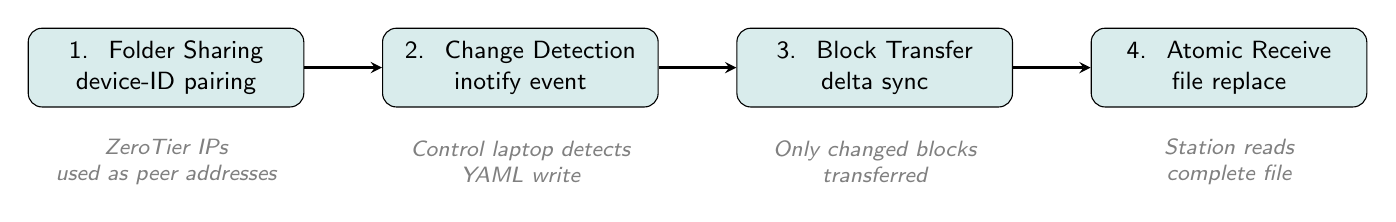
\begin{tikzpicture}[
    font=\small\sffamily,
    flowstep/.style={
        draw, rounded corners=5pt, fill=teal!15,
        minimum width=3.5cm, minimum height=1cm,
        align=center, text width=3.2cm
    },
    arrow/.style={->, >=stealth, thick},
    note/.style={font=\footnotesize\sffamily\itshape, text=gray, align=center}
]

% Steps in a row
\node[flowstep] (s1) at (0,0)     {1.\; Folder Sharing\\device-ID pairing};
\node[flowstep] (s2) at (4.5,0)   {2.\; Change Detection\\inotify event};
\node[flowstep] (s3) at (9,0)     {3.\; Block Transfer\\delta sync};
\node[flowstep] (s4) at (13.5,0)  {4.\; Atomic Receive\\file replace};

\draw[arrow] (s1) -- (s2);
\draw[arrow] (s2) -- (s3);
\draw[arrow] (s3) -- (s4);

% Notes below each step
\node[note] at (0,-1.2)    {ZeroTier IPs\\used as peer addresses};
\node[note] at (4.5,-1.2)  {Control laptop detects\\YAML write};
\node[note] at (9,-1.2)    {Only changed blocks\\transferred};
\node[note] at (13.5,-1.2) {Station reads\\complete file};

\end{tikzpicture}
\caption{Syncthing program-storage transfer lifecycle.}
\label{fig:ch6_syncthing_flow}
\end{figure}

Key properties of the Syncthing channel that complement the DDS real-time channel are:

\begin{itemize}
    \item \textbf{Automatic resumption.}  If the ZeroTier link drops during a transfer, Syncthing
          resumes from the last acknowledged block once connectivity is restored, so the station
          never reads a partially written file.

    \item \textbf{Versioning.}  Syncthing maintains a configurable number of previous file revisions,
          enabling rollback to an earlier validated program if an operator commits a bad plan.

    \item \textbf{Zero extra infrastructure.}  Syncthing establishes its encrypted TLS connection
          directly to the peer ZeroTier address — no cloud relay or additional server is needed.
\end{itemize}

% ------------------------------------------------------------------
\subsection{Two-Channel Message Flow Summary}
\label{subsec:ch6_flow_summary}
% ------------------------------------------------------------------

Figure~\ref{fig:ch6_full_flow} combines both channels and all payloads into a single reference
diagram, illustrating the directional asymmetry of the exchange.

% ------------------------------------------------------------------
%  Figure: complete two-channel data-flow diagram (TikZ)
% ------------------------------------------------------------------
\begin{figure}[H]
\centering
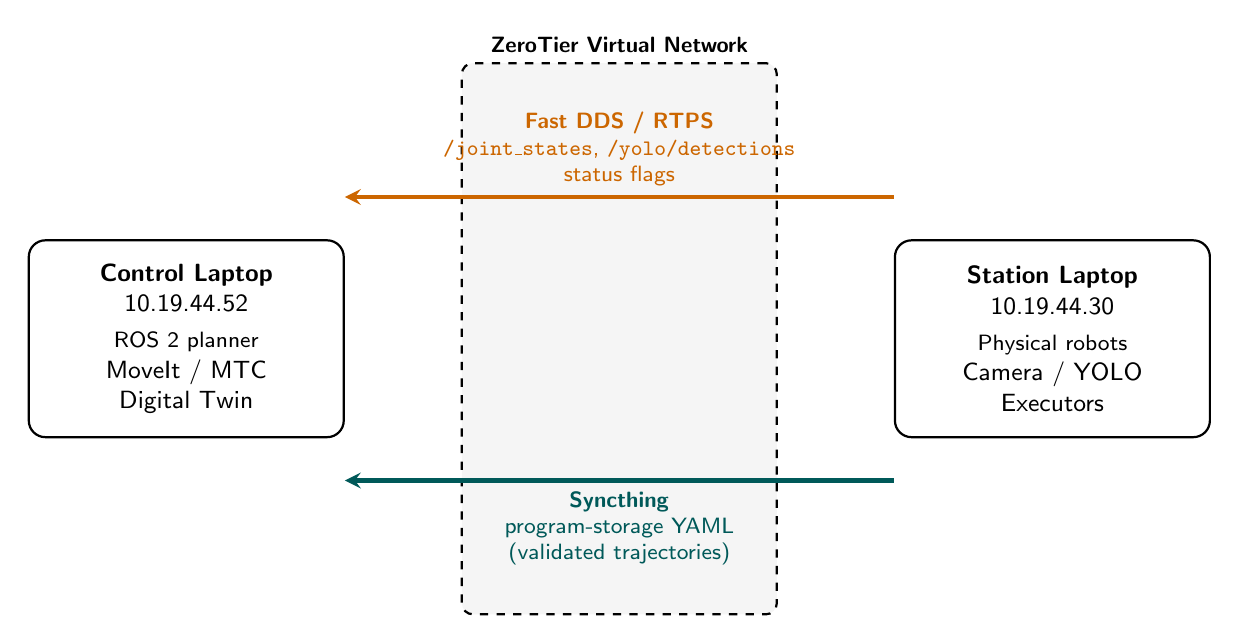
\begin{tikzpicture}[
    font=\small\sffamily,
    laptop/.style={
        draw, thick, rounded corners=6pt,
        minimum width=4cm, minimum height=2.5cm,
        align=center, fill=white
    },
    channel/.style={draw, thick, dashed, rounded corners=4pt,
        fill=gray!8, inner sep=8pt},
    msg/.style={->, >=stealth, thick},
    rmsg/.style={<-, >=stealth, thick},
    lbl/.style={font=\footnotesize\sffamily, align=center}
]

% Laptops
\node[laptop] (ctrl) at (-5.5, 0) {%
    \textbf{Control Laptop}\\10.19.44.52\\[2pt]
    \footnotesize ROS~2 planner\\MoveIt / MTC\\Digital Twin};

\node[laptop] (stat) at (5.5, 0) {%
    \textbf{Station Laptop}\\10.19.44.30\\[2pt]
    \footnotesize Physical robots\\Camera / YOLO\\Executors};

% ZeroTier bubble
\node[channel, minimum width=4cm, minimum height=7cm] (zt) at (0,0) {};
\node[font=\footnotesize\bfseries\sffamily, above] at (zt.north) {ZeroTier Virtual Network};

% Fast DDS arrow (upward stream – station to control)
\draw[msg, color=orange!80!black, line width=1.5pt]
    ([yshift=1.8cm] stat.west) -- node[above, lbl, color=orange!80!black]{%
        \textbf{Fast DDS / RTPS}\\
        \texttt{/joint\_states},
        \texttt{/yolo/detections}\\
        status flags}
    ([yshift=1.8cm] ctrl.east);

% Syncthing arrow (downward stream – control to station)
\draw[rmsg, color=teal!70!black, line width=1.5pt]
    ([yshift=-1.8cm] ctrl.east) -- node[below, lbl, color=teal!70!black]{%
        \textbf{Syncthing}\\
        program-storage YAML\\
        (validated trajectories)}
    ([yshift=-1.8cm] stat.west);

\end{tikzpicture}
\caption{Complete two-channel communication architecture.}
\label{fig:ch6_full_flow}
\end{figure}

The two-channel design cleanly separates concerns: time-critical, high-rate telemetry travels
on the DDS link where per-message QoS contracts are available, while the infrequently updated
program file is handled by a service purpose-built for reliable, resumable file delivery.
Together they provide the full communication backbone required by the distributed
digital-twin-enabled robotic cell.